\documentclass[11pt,a4paper]{article}
\usepackage[utf8]{inputenc}
\usepackage[spanish]{babel}
\usepackage{amsmath}
\usepackage{amsfonts}
\usepackage{amssymb}
\usepackage[export]{adjustbox}
\usepackage{tabularx}
\usepackage[table]{xcolor}
\usepackage{float}
\usepackage{url}
\usepackage{hyperref}
\hypersetup{
    colorlinks=true,
    linkcolor=black,
    filecolor=black,      
    urlcolor=blue,
    citecolor=blue,
}
\usepackage{graphicx}
\graphicspath{ {images/} }


\begin{document}


\begin{titlepage}

\includegraphics[scale=0.2,right,valign=t]{uoc-logo.png}
\vspace*{\fill}
\begin{flushleft}
{\LARGE \textbf{YouTubeCrawlerTool: Obtención de Big Data destinado al estudio del movimiento antivacuna haciendo crawler sobre YouTube}}
\end{flushleft}
\begin{flushleft}
\textbf{Javier Sánchez Mendoza}\\
Grado de ingeniería informática\\
Health IT
\end{flushleft}
\begin{flushleft}
\textbf{Carlos Luis Sánchez Bocanegra}\\
\textbf{José Antonio Morán Moreno}
\end{flushleft}
\begin{flushleft}
27 de marzo de 2018  
\end{flushleft}
\end{titlepage}


\begin{titlepage}
\vspace*{\fill}
\begin{flushleft}

\includegraphics[scale=1,left]{licencia-cc.png}
Esta obra está sujeta a una licencia de\\
Reconocimiento-NoComercial-SinObraDerivada\\
\href{http://creativecommons.org/licenses/by-nc-nd/3.0/es/}{3.0 España de Creative Commons}
\end{flushleft}
\end{titlepage}


\begin{center}
\textbf{FICHA DEL TRABAJO FINAL}
\end{center}
\begin{tabularx}{\textwidth}{|X|X|}
\hline 
\textbf{Título del trabajo:} &\cellcolor{gray!25} \textit{YouTubeCrawlerTool: Obtención de Big Data destinado al estudio del movimiento antivacuna haciendo crawler sobre YouTube} \\ 
\hline 
\textbf{Nombre del autor:} &\cellcolor{gray!25} \textit{Javier Sánchez Mendoza} \\ 
\hline 
\textbf{Nombre del consultor/a:} &\cellcolor{gray!25} \textit{Carlos Luis Sánchez Bocanegra} \\ 
\hline 
\textbf{Nombre del PRA:} &\cellcolor{gray!25} \textit{José Antonio Morán Moreno} \\ 
\hline 
\textbf{Fecha de entrega (mm/aaaa):} &\cellcolor{gray!25} \textit{MM/AAAA} \\ 
\hline 
\textbf{Titulación:} &\cellcolor{gray!25} \textit{Grado de ingeniería informática} \\ 
\hline 
\textbf{Área del Trabajo Final:} &\cellcolor{gray!25} \textit{Health IT} \\ 
\hline 
\textbf{Idioma del trabajo:} &\cellcolor{gray!25} \textit{Español} \\ 
\hline 
\textbf{Palabras clave:} &\cellcolor{gray!25} \textit{Big data, crawler, YouTube.} \\ 
\hline
\end{tabularx} 
\begin{tabularx}{\textwidth}{|X|}
\textbf{Resumen del Trabajo (máximo 250 palabras):} \textit{Con la finalidad, contexto de aplicación, metodología, resultados i conclusiones del trabajo.} \\ 
\hline 
\cellcolor{gray!25} \textit{...} \\
\hline 
\end{tabularx} 
\newpage 


\begin{tabularx}{\textwidth}{|X|}
\hline 
\textbf{Abstract (in English, 250 words or less):} \\ 
\hline 
\cellcolor{gray!25} \textit{...} \\
\hline 
\end{tabularx} 
\newpage 


\tableofcontents
\newpage


\listoffigures
\newpage


\section{Introducción}
En esta sección se detalla el proyecto, la motivación de la elección de la temática escogida y la planificación y estructuración del mismo.

\subsection{Contexto y justificación del Trabajo}
Desde la introducción de la vacunación como método preventivo de enfermedades han existido entidades y grupos de personas que se han opuesto a ella y han dudado de su efectividad o propósito \cite{1}. Hoy en día el activismo anti-vacunación (conocido también como movimiento antivacunas) ha vuelto a la actualidad y se encuentra en auge en algunas regiones tales como Europa o Estados Unidos, cobrándose en el peor de los escenarios victimas mortales a causa de enfermedades que se creían erradicadas y que han vuelto a surgir \cite{2}\cite{3}. 

Para hacer posible el estudio y comprensión de las motivaciones del movimiento antivacuna se propone el desarrollo de una aplicación que permita la recolección de grandes cantidades de datos de la actividad realizada por parte de este colectivo en la red social \textit{YouTube} con el fin de habilitar su posterior tratamiento y estudio por parte de una analista de datos (\textit{data scientist} \cite{4}) en el desarrollo de su trabajo final de master. 
\linebreak

Proyecto que se enmarca dentro de la problemática de la obtención, almacenamiento y procesamiento de grandes volúmenes de datos (\textit{Big Data} \cite{5}).
\linebreak

Hoy en día las redes sociales han puesto al alcance de los analistas de datos una gran cantidad de datos disponibles para ser analizados, una de las problemáticas a las que se quiere hacer frente es la obtención de dichos datos de forma efectiva. Para ello se propone hacer uso de interfaces de programación de aplicaciones (abreviado como \textit{API} \cite{6} en ingles) ofrecidas públicamente por \textit{YouTube} de tal forma que el proceso resulte transparente para el usuario final, en nuestro caso una analista de datos, permitiéndole la extracción a este problema. 

La obtención de grandes volúmenes de datos nos llevara también a la problemática que surge en su almacenamiento en bases de datos tradicionales y su posterior procesamiento. Para habilitar al usuario final el correcto acceso a la información obtenida se estudiaran las ventajas que aporta el uso de bases de datos \textit{NoSQL} \cite{7} para este cometido, al ser diseñadas especialmente para manejar enormes cantidades de datos.

\subsection{Objetivos del Trabajo}
El principal objetivo del proyecto es el de proporcionar una aplicación web que permita a una analista de datos obtener, de forma usable y transparente, la información que requiera de la red social \textit{YouTube} enfocado a realizar una investigación sobre el movimiento antivacunas.

Algunos de los objetivos concretos que se quieren lograr con este proyecto son los siguientes: 

\begin{itemize}
\item Investigar que funcionalidades aportan las \textit{API} públicas ofrecidas por \textit{YouTube} y analizar como se pueden utilizar para la obtención de la información requerida.
\item Determinar como almacenar y acceder de forma eficiente a la gran cantidad de información que se obtendrá.
\item Permitir la recolección de información según criterios de búsqueda proporcionados por el usuario final.
\item Habilitar la gestión, visualización y exportación de datos obtenidos en distintos procesos de extracción para su posterior análisis en herramientas especializadas.
\item Ofrecer herramientas de visualización para el análisis y comprensión de los datos obtenidos.
\item Proporcionar una interfaz de usuario usable que permita realizar las acciones requeridas por el usuario final.
\end{itemize}

\subsection{Enfoque y método seguido}
Para la realización del proyecto se seguirá el marco ágil de desarrollo \textit{scrum} \cite{8}. Al adoptar esta metodología como marco de trabajo nos permitirá, a diferencia de otras metodologías lineales de desarrollo como pueden ser los modelos en cascada, poder desarrollar el proyecto de forma flexible permitiéndonos adaptar la planificación inicial del proyecto en caso de ser necesario para adecuarse a nuevos requerimientos.

La forma en la cual se aplicara la metodología \textit{scrum} en el proyecto esta condicionada por los integrantes del equipo de desarrollo, en el actual la figura del \textit{product owner}, \textit{scrum master} y desarrollador recaerán sobre la figura del alumno que presenta el actual proyecto descrito (Javier Sánchez Mendoza), mientras que la figura del cliente estará representada por una analista de datos en el desarrollo de su trabajo final de master (Johanna Rodríguez) y el consultor de los mismos (Carlos Luis Sánchez Bocanegra) como \textit{stakeholder}.

Siguiendo la metodología \textit{scrum}, se realizaran iteraciones (comúnmente conocidos como \textit{sprints}) de una semana de duración donde, en la finalización de los mismos, se realizaran reuniones online para revisar y aprobar las tareas realizadas (\textit{sprint review}) y definir las tareas para la siguiente iteración (\textit{sprint planning}). Para gestionar las tareas a realizar (\textit{backlog}) se ha decidido utilizar la herramienta online \textit{Trello} \cite{9}:

\begin{figure}[hbtp]
\centering
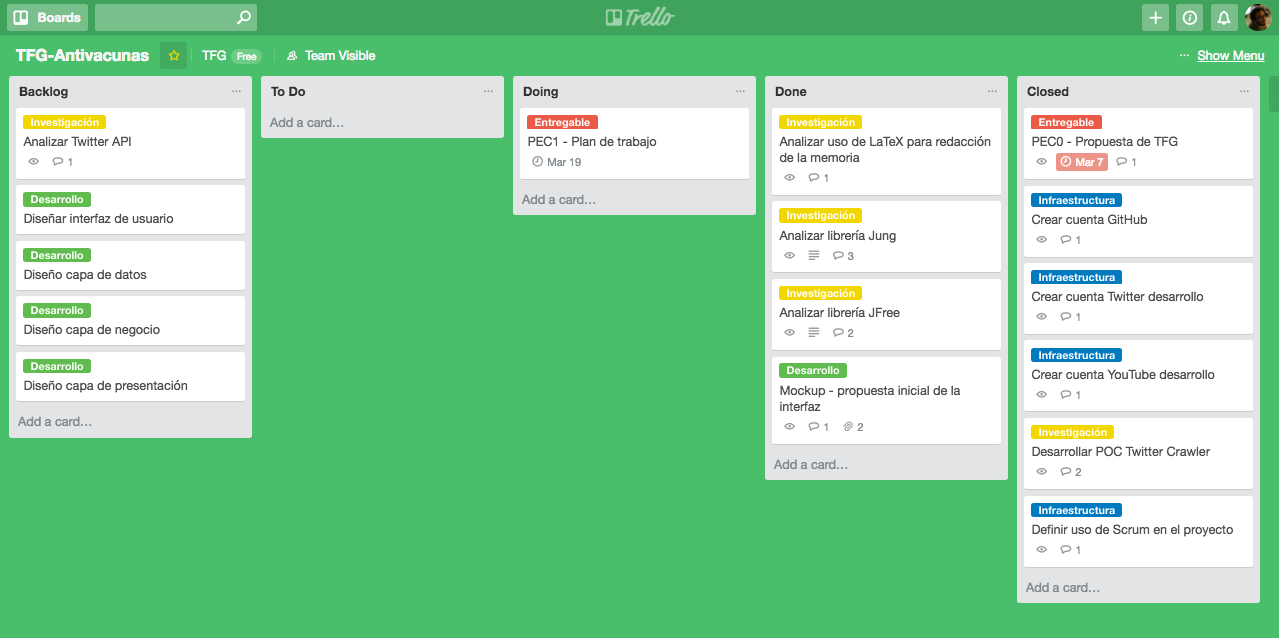
\includegraphics[scale=0.3]{planificacion/trello-backlog.png}
\caption{Ejemplo del backlog del proyecto en Trello}
\end{figure}

\subsection{Planificación del Trabajo}
En la realización del proyecto se seguirá la planificación detallada en el diagrama de \textit{Grantt} tentativo facilitado en las figuras dos, tres y cuatro. Cabe destacar que el diagrama proporcionado representa una estimación inicial de la planificación del proyecto y esta sujeto a modificaciones al inicio de cada iteración.

\begin{figure}[H]
\centering
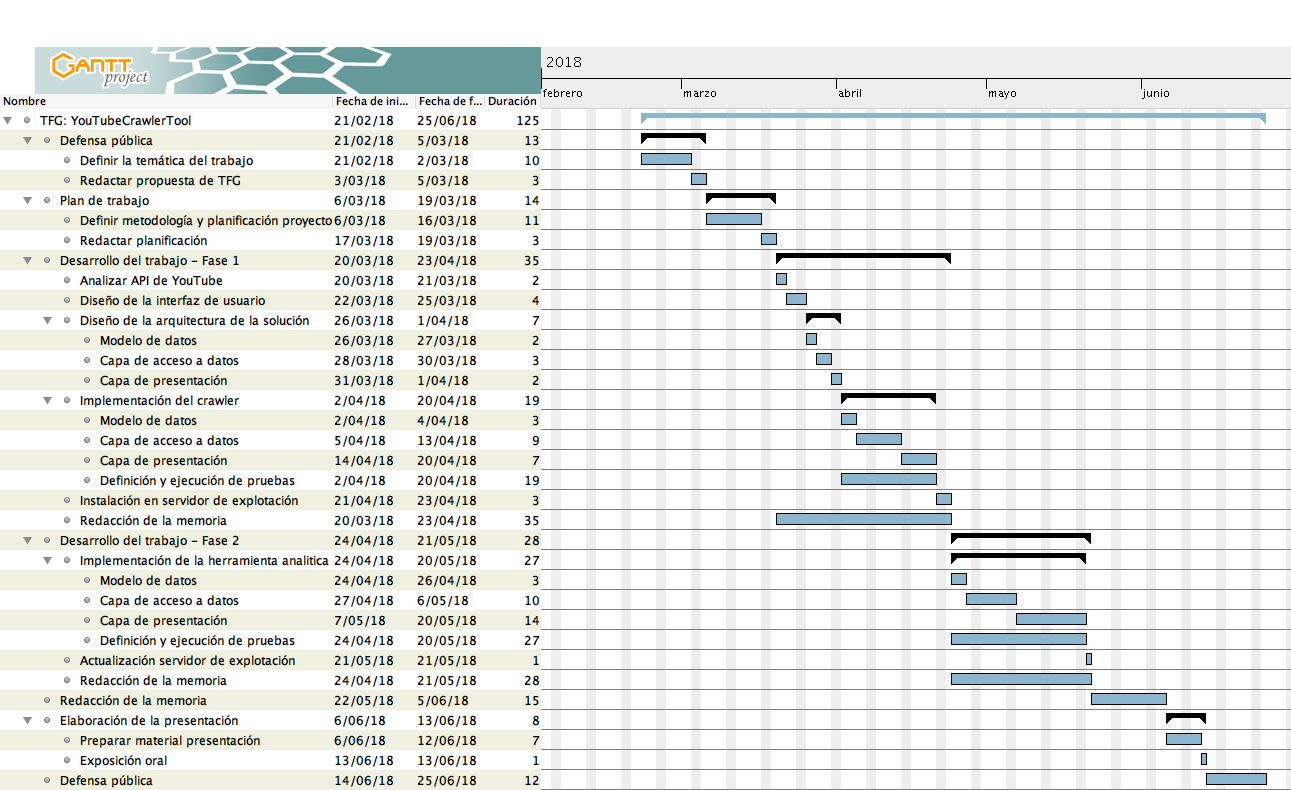
\includegraphics[scale=0.25]{planificacion/planificacion.png}
\caption{Listado de tareas y diagrama de Gantt}
\end{figure}

\begin{figure}[H]
\centering
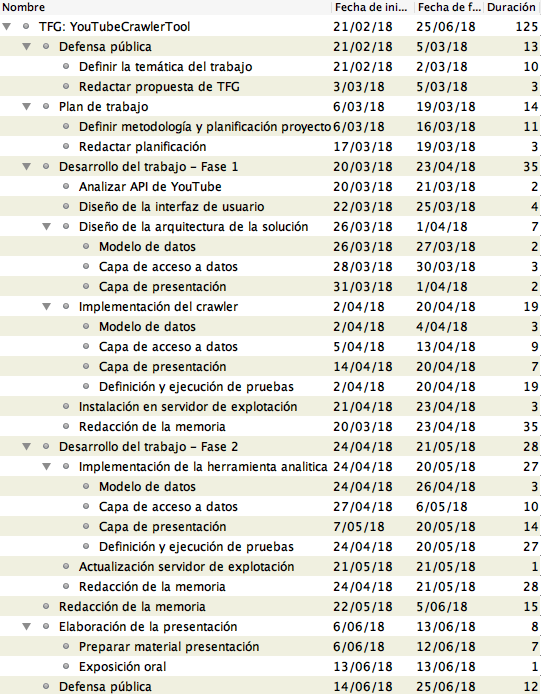
\includegraphics[scale=0.4]{planificacion/listado-tareas.png}
\caption{Listado de tareas}
\end{figure}

\begin{figure}[H]
\centering
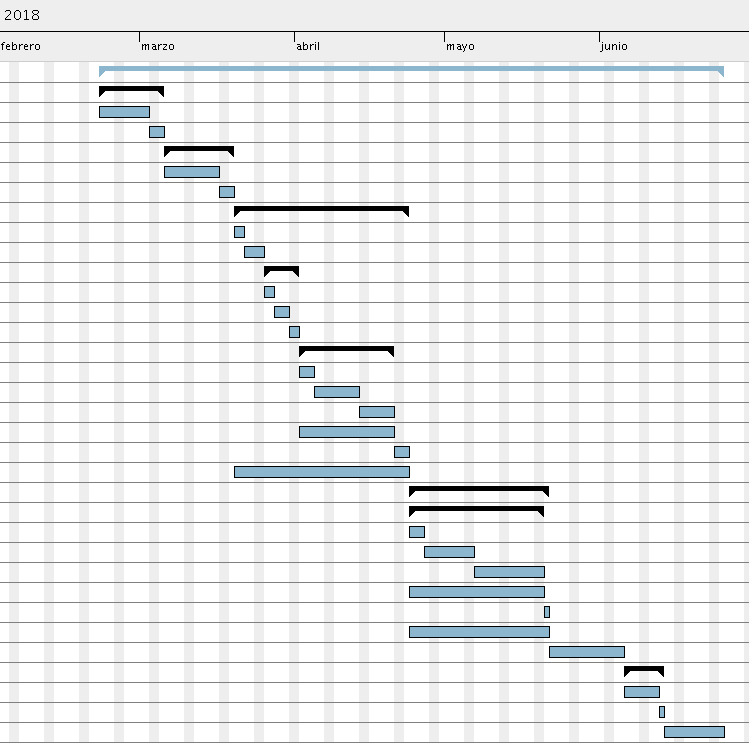
\includegraphics[scale=0.3]{planificacion/diagrama-gantt.png}
\caption{Diagrama de Gantt}
\end{figure}

De la planificación facilitada cabe destacar que la redacción de la memoria se ha diseñado como una tarea evolutiva que se ira desarrollando durante todas las fases del proyecto pero mas intensamente durante la antepenúltima fase dedicada exclusivamente a su redacción. Además, durante las dos fases de desarrollo se han planificado dos tareas recurrentes para la definición y realización de pruebas de calidad del producto a realizar durante todo el ciclo de desarrollo.

Como se puede observar, en el diagrama facilitado en cada entrega se espera conseguir unos hitos concretos. La relación de los mas destacables por entrega son los siguientes:

\begin{itemize}
\item \textbf{Definición de los contenidos del trabajo:} Redacción propuesta TFG.
\item \textbf{Plan de trabajo:} Redacción planificación.
\item \textbf{Desarrollo del trabajo – Fase 1:} Instalación en servidor de explotación de la primera versión de la aplicación con funcionalidad de \textit{crawler} implementada.
\item \textbf{Desarrollo del trabajo – Fase 2:} Actualización en servidor de explotación de la versión final de la aplicación con funcionalidad analítica implementada.
\item \textbf{Redacción de la memoria:} Entrega de la memoria del proyecto.
\item \textbf{Elaboración de la presentación:} Realizar exposición oral.
\item \textbf{Defensa pública:} Defender públicamente el proyecto.
\end{itemize}

Los riesgos detectados en la planificación se concentran principalmente en la consecución del hito definido en la primera fase de desarrollo. Para permitir al cliente de la aplicación poder empezar a recopilar datos para su investigación lo antes posible, se ha decidido realizar la instalación de la aplicación desarrollada en entorno de explotación en dos fases distintas, una con la funcionalidad del \textit{crawler} y otra con la funcionalidad analítica implementada. La demora en la primera fase de desarrollo podría comprometer el éxito de la investigación del cliente. Para mitigar este riesgo se realizara el seguimiento del mismo durante las diferentes iteraciones en esta fase de desarrollo y de ser necesario se tomaran conjuntamente con el cliente las acciones correctoras requeridas. 


\subsection{Breve sumario de productos obtenidos}
No hay que entrar en detalle: la descripción detallada se hará en el resto de capítulos. 

\subsection{Breve descripción de los otros capítulos de la memoria}
Explicación de los contenidos de cada capítulo y su relación con el trabajo en global.
\newpage 


\section{Resto de capítulos}
En estos capítulos, hay que describir los aspectos más relevante del diseño y desarrollo del proyecto, así como de los productos obtenidos. La estructuración de los capítulos puede variar según el tipo de Trabajo.  

En cada apartado es muy importante describir las alternativas posibles, los criterios utilizados para tomar decisiones y la decisión tomada.

En caso de que corresponda, se incluirá un apartado de “Valoración económica del trabajo”. Este apartado indicará los gastos asociados al desarrollo y mantenimiento del trabajo, así como los beneficios económicos obtenidos. Hacer un análisis final sobre la viabilidad del producto. 
\newpage 


\section{Conclusiones}
Este capítulo tiene que incluir:
\begin{itemize}
\item Una descripción de las conclusiones del trabajo: Qué lecciones se han aprendido del trabajo?.
\item Una reflexión crítica sobre el logro de los objetivos planteados inicialmente: Hemos logrado todos los objetivos? Si la respuesta es negativa, por qué motivo? 
\item Un análisis crítico del seguimiento de la planificación y metodología a lo largo del producto: Se ha seguido la planificación? La metodología prevista ha sido la adecuada? Ha habido que introducir cambios para garantizar el éxito del trabajo? Por qué? 
\item Las líneas de trabajo futuro que no se han podido explorar en este trabajo y han quedado pendientes.
\end{itemize}
\newpage 


\section{Glosario}
Definición de los términos y acrónimos más relevantes utilizados dentro de la Memoria. 
\newpage 


\section{Bibliografía}
\begin{thebibliography}{0}
  \bibitem{1} \url{https://es.wikipedia.org/wiki/Controversia_de_las_vacunas} (07/03/2018)
  \bibitem{2} \url{http://www.elmundo.es/cataluna/2015/06/27/558e5fb2e2704ea41e8b4576.html} (07/03/2018)
  \bibitem{3} \url{https://buenavibra.es/movida-sana/salud/italia-sarampion-movimientos-antivacunas} (16/03/2018)
  \bibitem{4} \url{https://es.wikipedia.org/wiki/Ciencia_de_datos} (07/03/2018)
  \bibitem{5} \url{https://es.wikipedia.org/wiki/Macrodatos} (07/03/2018)
  \bibitem{6} \url{https://es.wikipedia.org/wiki/Interfaz_de_programacion_de_aplicaciones} (07/03/2018)
  \bibitem{7} \url{https://es.wikipedia.org/wiki/NoSQL} (07/03/2018)
  \bibitem{8} \url{https://es.wikipedia.org/wiki/Scrum_(desarrollo_de_software)} (16/03/2018)
  \bibitem{9} \url{https://trello.com} (16/03/2018)
\end{thebibliography}
\newpage 


\section{Anexos}
Listado de apartados que son demasiado extensos para incluir dentro de la memoria y tienen un carácter autocontienido (por ejemplo, manuales de usuario, manuales de instalación, etc.) 

Dependiente del tipo de trabajo, es posible que no haya que añadir ningún anexo.

\end{document}
